\chapter{Introduction}

Suppose you have a small dataset and need to train a model for some task, say classification.
% How would you go about doing it?
A pipeline that has become standard today is to download the latest pre-trained deep network and fine-tune it on your own small dataset. This pre-trained model used to be ImageNet-based~\cite{deng2009imagenet,he2016deep} and now would probably be CLIP~\cite{radford2021learning}. The implicit goal set by the community for such pre-trained models is that they should transfer well to any kind of downstream task not known in advance. This has led to a race to build ultra-large-scale models in terms of computation, model size, and dataset size. But is this goal of building an ``omniscient'' pre-trained model that can work on any future downstream task even feasible? Perhaps not because our world is continually changing.
Although the size of the pretraining datasets has grown from 1.2M~~\cite{deng2009imagenet} to 400M~\cite{schuhmann2021laion} images, what has not changed at all is their nature: these datasets are curated, and, more importantly, \textit{\textbf{static}}. For instance, the portion of ImageNet curated before 2007 has no idea what an iPhone is.
% "static": Jason, to me, this is the most important part of the motivation. size of the dataset is not that important since we already have such big datasets that we only train 1-2 epochs on. the main issue with these datasets is that they are fixed in time. ontologies change rapidly (eg new products come out), category meanings might change (eg what a smartphone looks like is different in 2023 vs 2013), new words may even develop (eg slay). I think the focus should be on training a static dataset by design will produce an outdated model. this isn't really mentioned until paragraph 2 and stays kinda vague
Furthermore, although a few hundred million images represent a staggering quantity of visual data, they are minuscule compared to the entire Internet, where billions of new photos are uploaded every day.
% , continuously updating with an incredible diversity of real-world objects and scenes.
Thus, current static datasets, however big they become,
% , are minuscule compared to the entire Internet, where billions of new photos are uploaded every day. They
fail to capture the richness and dynamic nature of the data available on the Internet.
% Not to mention the issue that the bigger we make our static pre-training datasets, the more compute burden they entail.
% that the compute scales with the size of the dataset as well.
Moreover, as our static datasets grow, they require increasingly inaccessible amounts of compute.

% So the ``big data'' in machine learning is easily dwarfed by the data generated collectively by the world. Furthermore, the bigger we make our static pre-training datasets, the more compute burden they entail: e.g., CLIP is trained on 256 GPUs for 12 days. 
% This begs the question: \textit{are static datasets, as big as they are, ever going to truly scale to capture the richness and dynamic nature of the data available on the Internet? }
% This begs the question: \textit{will static datasets, however big they become, ever truly scale to capture the richness and dynamic nature of the data available on the Internet? }
% We suspect that the answer is no, so what could be the alternative? % want to remove this sentence

\begin{figure}[t]
    \centering
    % \includegraphics{figures/fig1-cvpr-2022v3.pdf}
    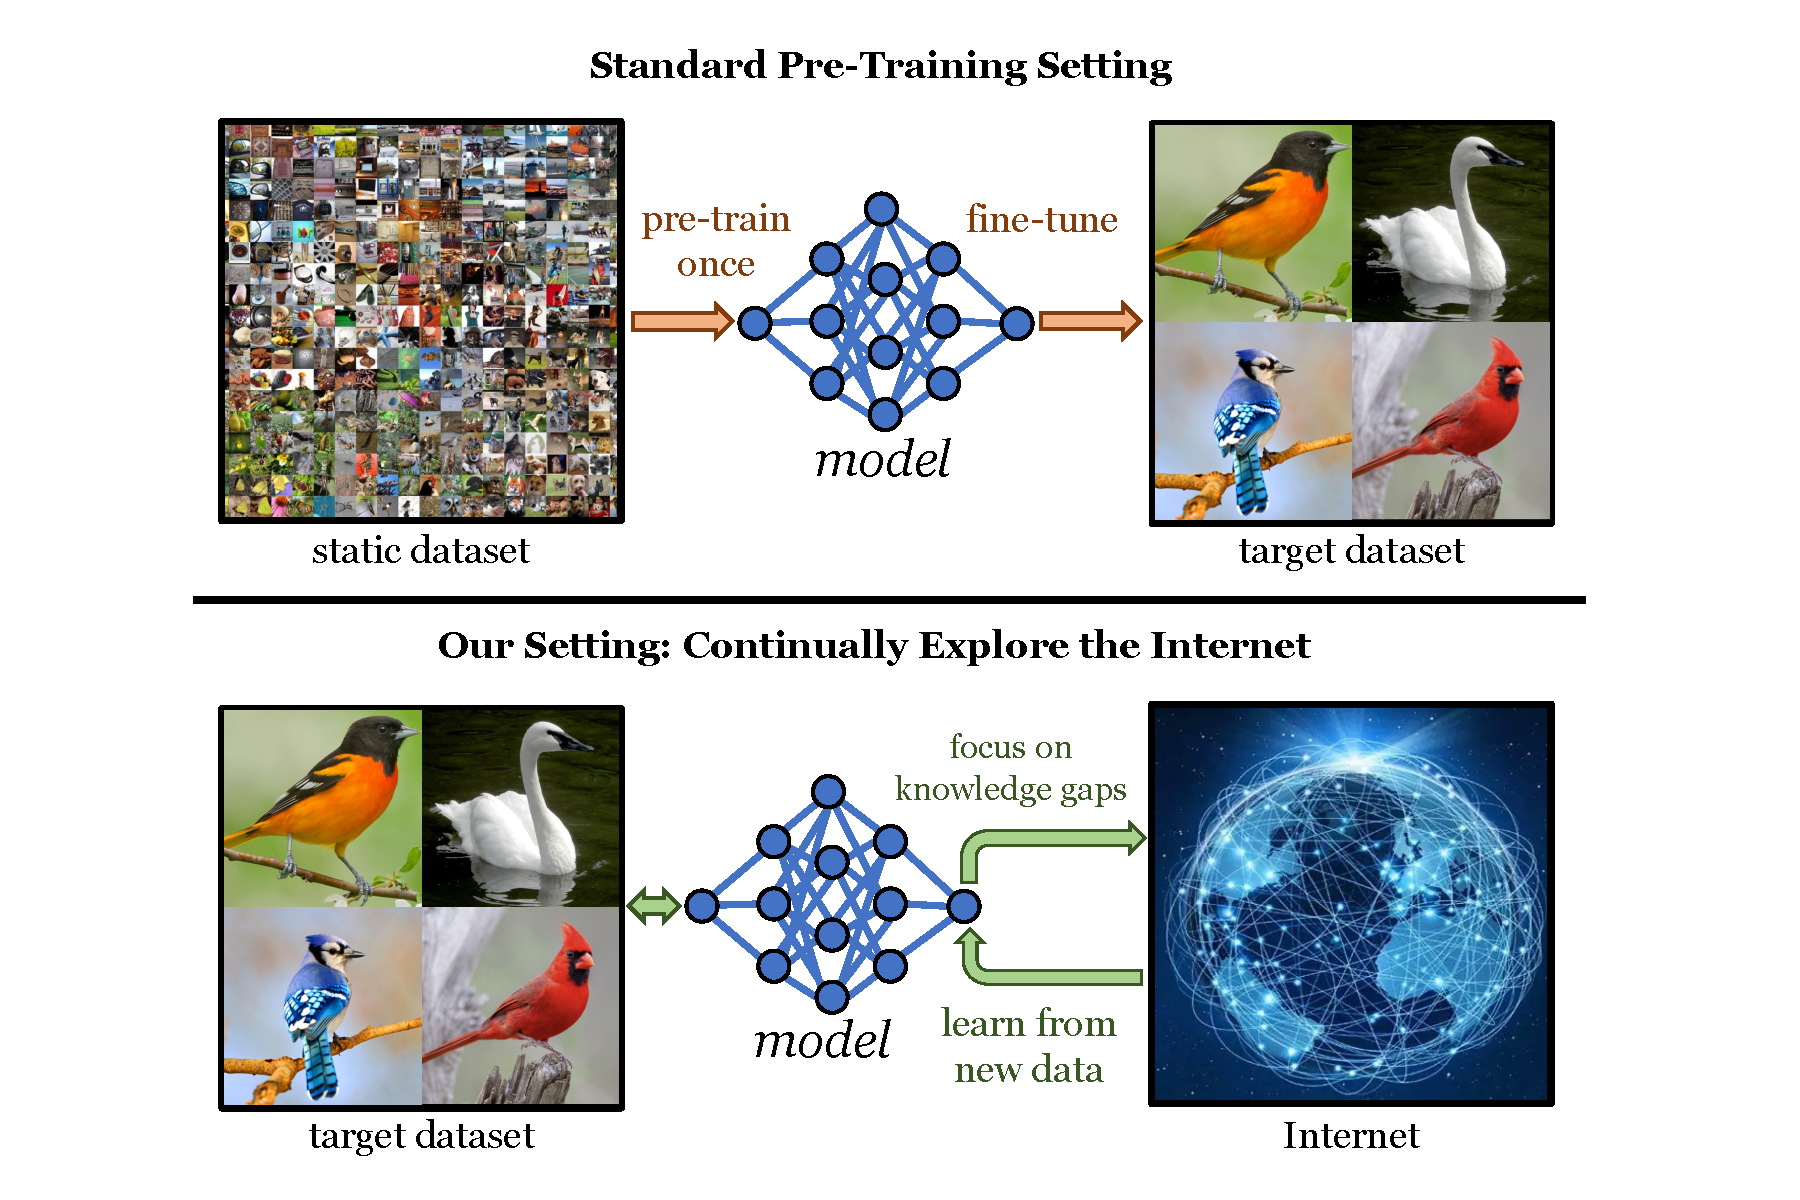
\includegraphics[width=0.8\linewidth]{figures/teaser2.pdf}
    % 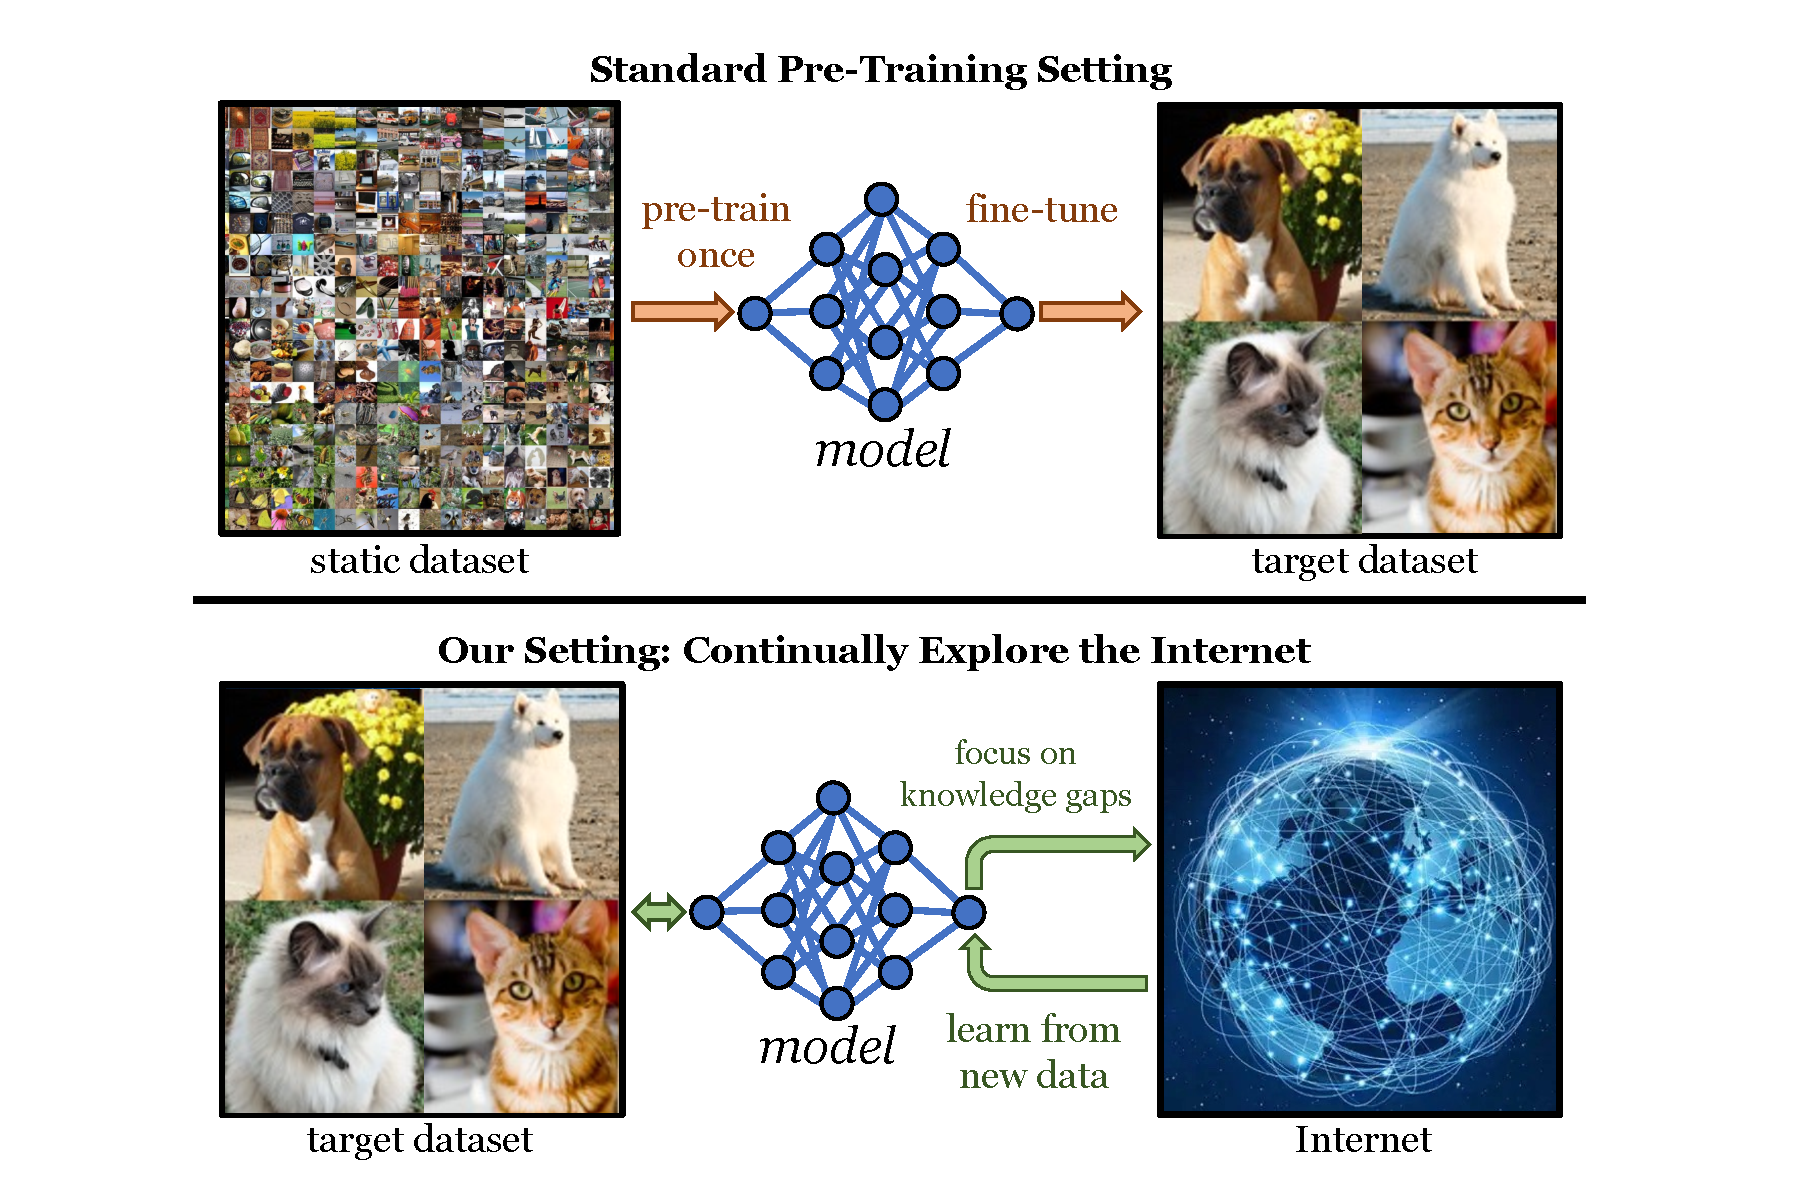
\includegraphics[width=\linewidth]{figures/alex.pdf}
    \caption{Given unlabeled data for a target task, our approach, Internet Explorer, searches the Internet to progressively find more and more relevant training data via self-supervised exploration.}
    \label{fig:teaser}
    % \vspace{-0.1in}
    \vspace{-0.15in}
\end{figure}

In this thesis, we rethink the idea of a \textit{\textbf{generic}} large-scale pretrained model and propose an alternate paradigm of training a rather small-scale but up-to-date model geared towards the \textit{\textbf{specific}} downstream task of interest. To train such a model, we go beyond static datasets and \textit{treat the Internet itself as a dynamic, open-ended dataset}. Unlike conventional datasets, which are expensive to increase and grow stale with time,
%are prone to bias, and yield suboptimal transfer performance when they contain little relevant data to the downstream task. 
the Internet is dynamic, rich, grows automatically, and is always up to date.
Its continuously evolving nature also means we cannot hope to ever download it or train a model, whether large or small, on all of it.
% But thinking pragmatically, do we even need to do so? Perhaps not.

We propose that the Internet can be treated as a special kind of dataset---one that exists out there, ready to be queried as needed to quickly train a customized model for a desired task.
% However, the issue is that the Internet is too big, and finding relevant images that help improve performance on a target dataset is a challenging endeavor.
We draw an analogy to reinforcement learning, where even though the task is known, finding a policy that can generate the desired behavior is non-trivial due to the high complexity of the state space. Hence, most approaches rely on some form of exploration to figure out what actions the agent should take so that it quickly finds high-reward states. Inspired by this analogy, we formulate a disembodied, online agent we call {\em Internet Explorer}, that actively searches the Internet using standard search engines to find relevant visual data that improve feature quality on a target dataset (see \cref{fig:teaser}). The agent's actions are text queries made to search engines, and the observations are the data obtained from the search.

The queries made by Internet Explorer improve over time. It cycles between searching for images on the Internet with text queries, self-supervised training on downloaded images, determining which images are relevant to the target dataset, and prioritizing what to search for next (see \cref{fig:method}). We also bootstrap Internet Explorer using existing pre-trained models such as MoCov3~\cite{he2020momentum} and obtain a significant boost on the target datasets.

Our setting is different from active learning~\cite{settles2009active}, where the goal is to selectively obtain labels for data points from a fixed dataset. In contrast, Internet Explorer continually expands the size of its dataset and requires no labels for training, even from the target dataset.
% However, we also show results in settings when the label set of the target dataset (not individual labels) are known.
Some prior works have also discussed ways to leverage the Internet as an additional source of data. NELL~\cite{carlson2010toward} proposed a way to continually scrape web pages to learn new concepts and relationships, which are periodically curated by a human in the loop. NEIL~\cite{chen2013neil} builds on the dictionary developed by NELL to search visual data to develop visual relationships. Both are semi-supervised methods to gather general ``common-sense'' knowledge from the Internet. In contrast, we perform an actively improving \textit{directed} search to perform well on target data, in a fully self-supervised manner. Recent work~\cite{jiang2021improving} follows a similar setting but searches a static dataset and not the Internet.

We evaluate Internet Explorer across 5 datasets, including 4 fine-grained datasets and PASCAL VOC.
% For simplicity, the search engine used is Google, but the method itself can work by searching on just image tags/captions as well.
We search for relevant images using Google; however, the method is compatible with any text-based search engine or even a static dataset (see \cref{subsec:search_engine_main}).
% \todo{prev sentence is out of date. mention laion / flickr}
We compare against several strong baselines, including CLIP, on downstream tasks. Note that CLIP acts as an oracle for our approach because it has likely already seen all or more queries that Internet Explorer makes.
In most scenarios, Internet Explorer either outperforms or matches CLIP oracle using only a single 3090 GPU desktop machine that runs for 30--40 hours, makes over 10K progressively improving queries, and downloads over 1M relevant Internet images for each target dataset.


\begin{figure}[t]
    \centering
    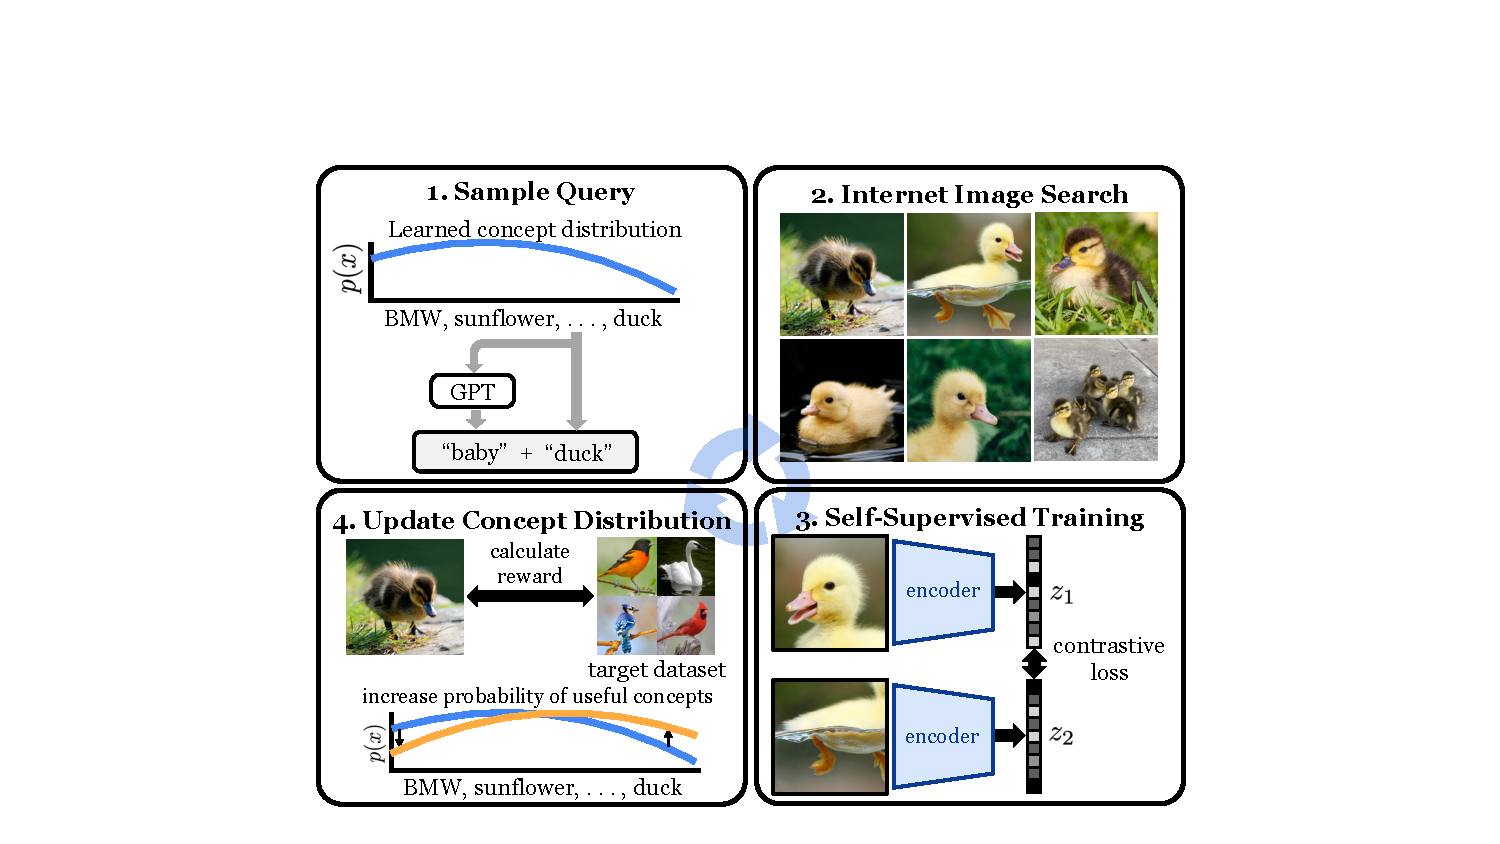
\includegraphics[width=0.85\linewidth]{figures/method_fig2.pdf}
    \caption{\textbf{Overview of Internet Explorer.} Our goal is to efficiently search the Internet for images that improve our performance on a target dataset.
        % In each iteration, we generate text queries by combining a concept sampled from a learned distribution with a GPT-generated descriptor. We query Google Images with the resulting phrase and download the top 100 image results. We add these images to the set of previously downloaded images and perform self-supervised learning on the combined dataset. 
        % Finally, we evaluate the relevance of the new images and increase the likelihood of the query and other related queries if the new images are similar to the target dataset.
        In each iteration, we first generate text queries by combining a concept sampled from a learned distribution with a GPT-generated descriptor (\S\ref{subsec:text_query_generation}, \ref{subsec:tiering}). Next, we query search engines with the resulting phrase and download the top 100 image results (\S\ref{subsec:text_to_image_search}, \ref{subsec:search_engine_main}). We add these images to the set of previously downloaded images and perform self-supervised training on the combined dataset (\S\ref{subsec:ssl}). Finally, we evaluate the relevance of the new images and update our concept distribution to increase the likelihood of similar queries if their images were similar to the target dataset (\S\ref{subsec:image_rel_reward},~\ref{subsec:unseen_reward}).
    }
    \label{fig:method}
    \vspace{-1em}
\end{figure}


%%% Local Variables:
%%% coding: utf-8
%%% mode: latex
%%% TeX-engine: xetex
%%% TeX-master: "../thesis"
%%% End: